\documentclass[12pt]{article}
%--------------------   start of the 'preamble'
%
\usepackage{graphicx,amssymb,amstext,amsmath,color}
\usepackage[margin=2cm]{geometry}
\usepackage{abstract}
\usepackage{setspace}
\usepackage[footnotesize,bf]{caption}

% TABLE
\usepackage{multicol,hhline,colortbl,multirow}
\usepackage{braket}
\usepackage{siunitx}
\usepackage{hyperref}
\usepackage{authblk}
\usepackage{siunitx}
\usepackage{mathrsfs}
%%\usepackage[sort&compress]{natbib}
%%\bibpunct{(}{)}{,}{a}{, }{;}
%
\usepackage[sort&compress]{natbib}
\bibpunct{[}{]}{,}{s}{}{;}


\definecolor{gray}{gray}{0.8}
\def\mobunits{\square\centi\meter\per\volt\per\second}
\def\gcm{\gram\per\cubic\centi\meter}
\def\ccg{\cellcolor{gray}}

\renewcommand{\labelitemii}{$\circ$}
\renewcommand{\bibname}{References}


\title{MorphCT Results - PCBM}
\author{Matthew Jones}
\date{\today}

\begin{document}
\maketitle

\section{Mobility Results}

\begin{center}
\begin{tabular}{| c | c | c | c | c | c |}
\hline
\rule{0pt}{2.5ex} 
\multirow{2}{*}{\textbf{ID}}&\multirow{2}{*}{\textbf{Simulation Name}}&\textbf{Density}&\textbf{Anisotropy}&\textbf{Anisotropy}&\textbf{Mobility}\\
&&(\SI{}{\gcm})&(Arb. U.)&(Shape)&(\SI{}{\mobunits})\\
\hhline{|======|}
\textbf{\ccg1}&\rule{0pt}{2.5ex}\ccg pcbm-0.5-P0.5-300-T3.0&\ccg 1.60&\ccg 0.0113&\ccg Spherical&\ccg4.05$\times 10^{-3}$\\
\textbf{2}&\rule{0pt}{2.5ex}pcbm-0.5-P0.5-200-T5.0&1.40&0.0394&Spherical&2.35$\times 10^{-2}$\\
\textbf{\ccg3}&\rule{0pt}{2.5ex}\ccg pcbm-0.5-P1.5-200-T3.0&\ccg 1.71&\ccg 0.0140&\ccg Spherical&\ccg1.58$\times 10^{-2}$\\
\textbf{4}&\rule{0pt}{2.5ex}pcbm-0.5-P1.5-200-T5.0&1.59&0.5107&Cigar&1.39$\times 10^{-1}$\\
\hhline{------}
\end{tabular}\label{table:mobResults}
\captionof{table}{MorphCT's latest results for the mobilities of pristine PCBM morphologies with a ball carbon C0A-C0A interaction strength, $\epsilon_{C0A-C0A} = 0.5 \mathcal{E}$, where $\mathcal{E} =$ \SI{1.4595E-21}{J}}
\end{center}

\subsection{Representative Values From Literature}
\begin{itemize}
    \item{Density: 1.40 - \SI{1.60}{\gcm}\cite{Arias2006,Kiel2010b,Bulle-Lieuwma2003}}
    \item{Mobility: \SI{1E-4}{} - \SI{1E-2}{\mobunits}\cite{Tuladhar2005}}
\end{itemize}

\begin{itemize}
    \item{Mobilities slightly high compared to literature, but within reasonable agreement.}
    \item{No clear density trend - \textbf{1} and \textbf{4} have the same densities but 2 orders of magnitude different mobilities.
        \begin{itemize}
            \item{However, the calculated density is just the film density. 
        It therefore doesn't take into account any of the voids in the simulation volume, which means that a higher density doesn't necessarily mean the fullerenes are closer together and therefore have better mobilities.}
        \end{itemize}}
    \item{Additionally, the mobilities do not follow the expected temperature trend at the same density ($\mu_{\textbf{1}} < \mu_{\textbf{4}}$ even though $T_{\textbf{1}} > T_{\textbf{4}}$).}
        \begin{itemize}
            \item{It is expected that the hotter morphology will be more disordered and therefore the mobility should be lower.
                    However, both $T_{\textbf{1}}$ and $T_{\textbf{4}}$ are below the melting temperature of a pure PCBM film, which is expected to be around \SI{550}{\kelvin}\cite{Ngo2012a}.
                Therefore it might not be exepected that there would be a significant difference in order between the two morphologies.}
            \item{While the above argument can reason why we might not expect $\mu_{\textbf{1}} > \mu_{\textbf{4}}$, it does not help explain the 2 order of magnitude discrepancy, nor the anisotropy results.}
        \end{itemize}
    \item{The anisotropies are approximately spherical for all of the simulations except $\textbf{4}$.
            \begin{itemize}
                \item{It is unlikely that the relative isotropic carrier motion of $\textbf{4}$ is a coincidence, especially when combined with its hight mobility.}
                \item{My hypothesis here is that the fullerenes are packing more closely along a particular axis in $\textbf{4}$ compared to the other morphologies, leading to high connectivity and transport along that route.
                    This would be visible in diffractometer results and visually more voids in the system off-axis, as the total film density is not significantly higher than in other systems.
                \textcolor{red}{EDIT: No significant difference in scattering patterns that highlights this difference.}}
            \end{itemize}}
\end{itemize}

\clearpage

\subsection{3D Carrier Network}

\begin{figure}[h!]\centering
	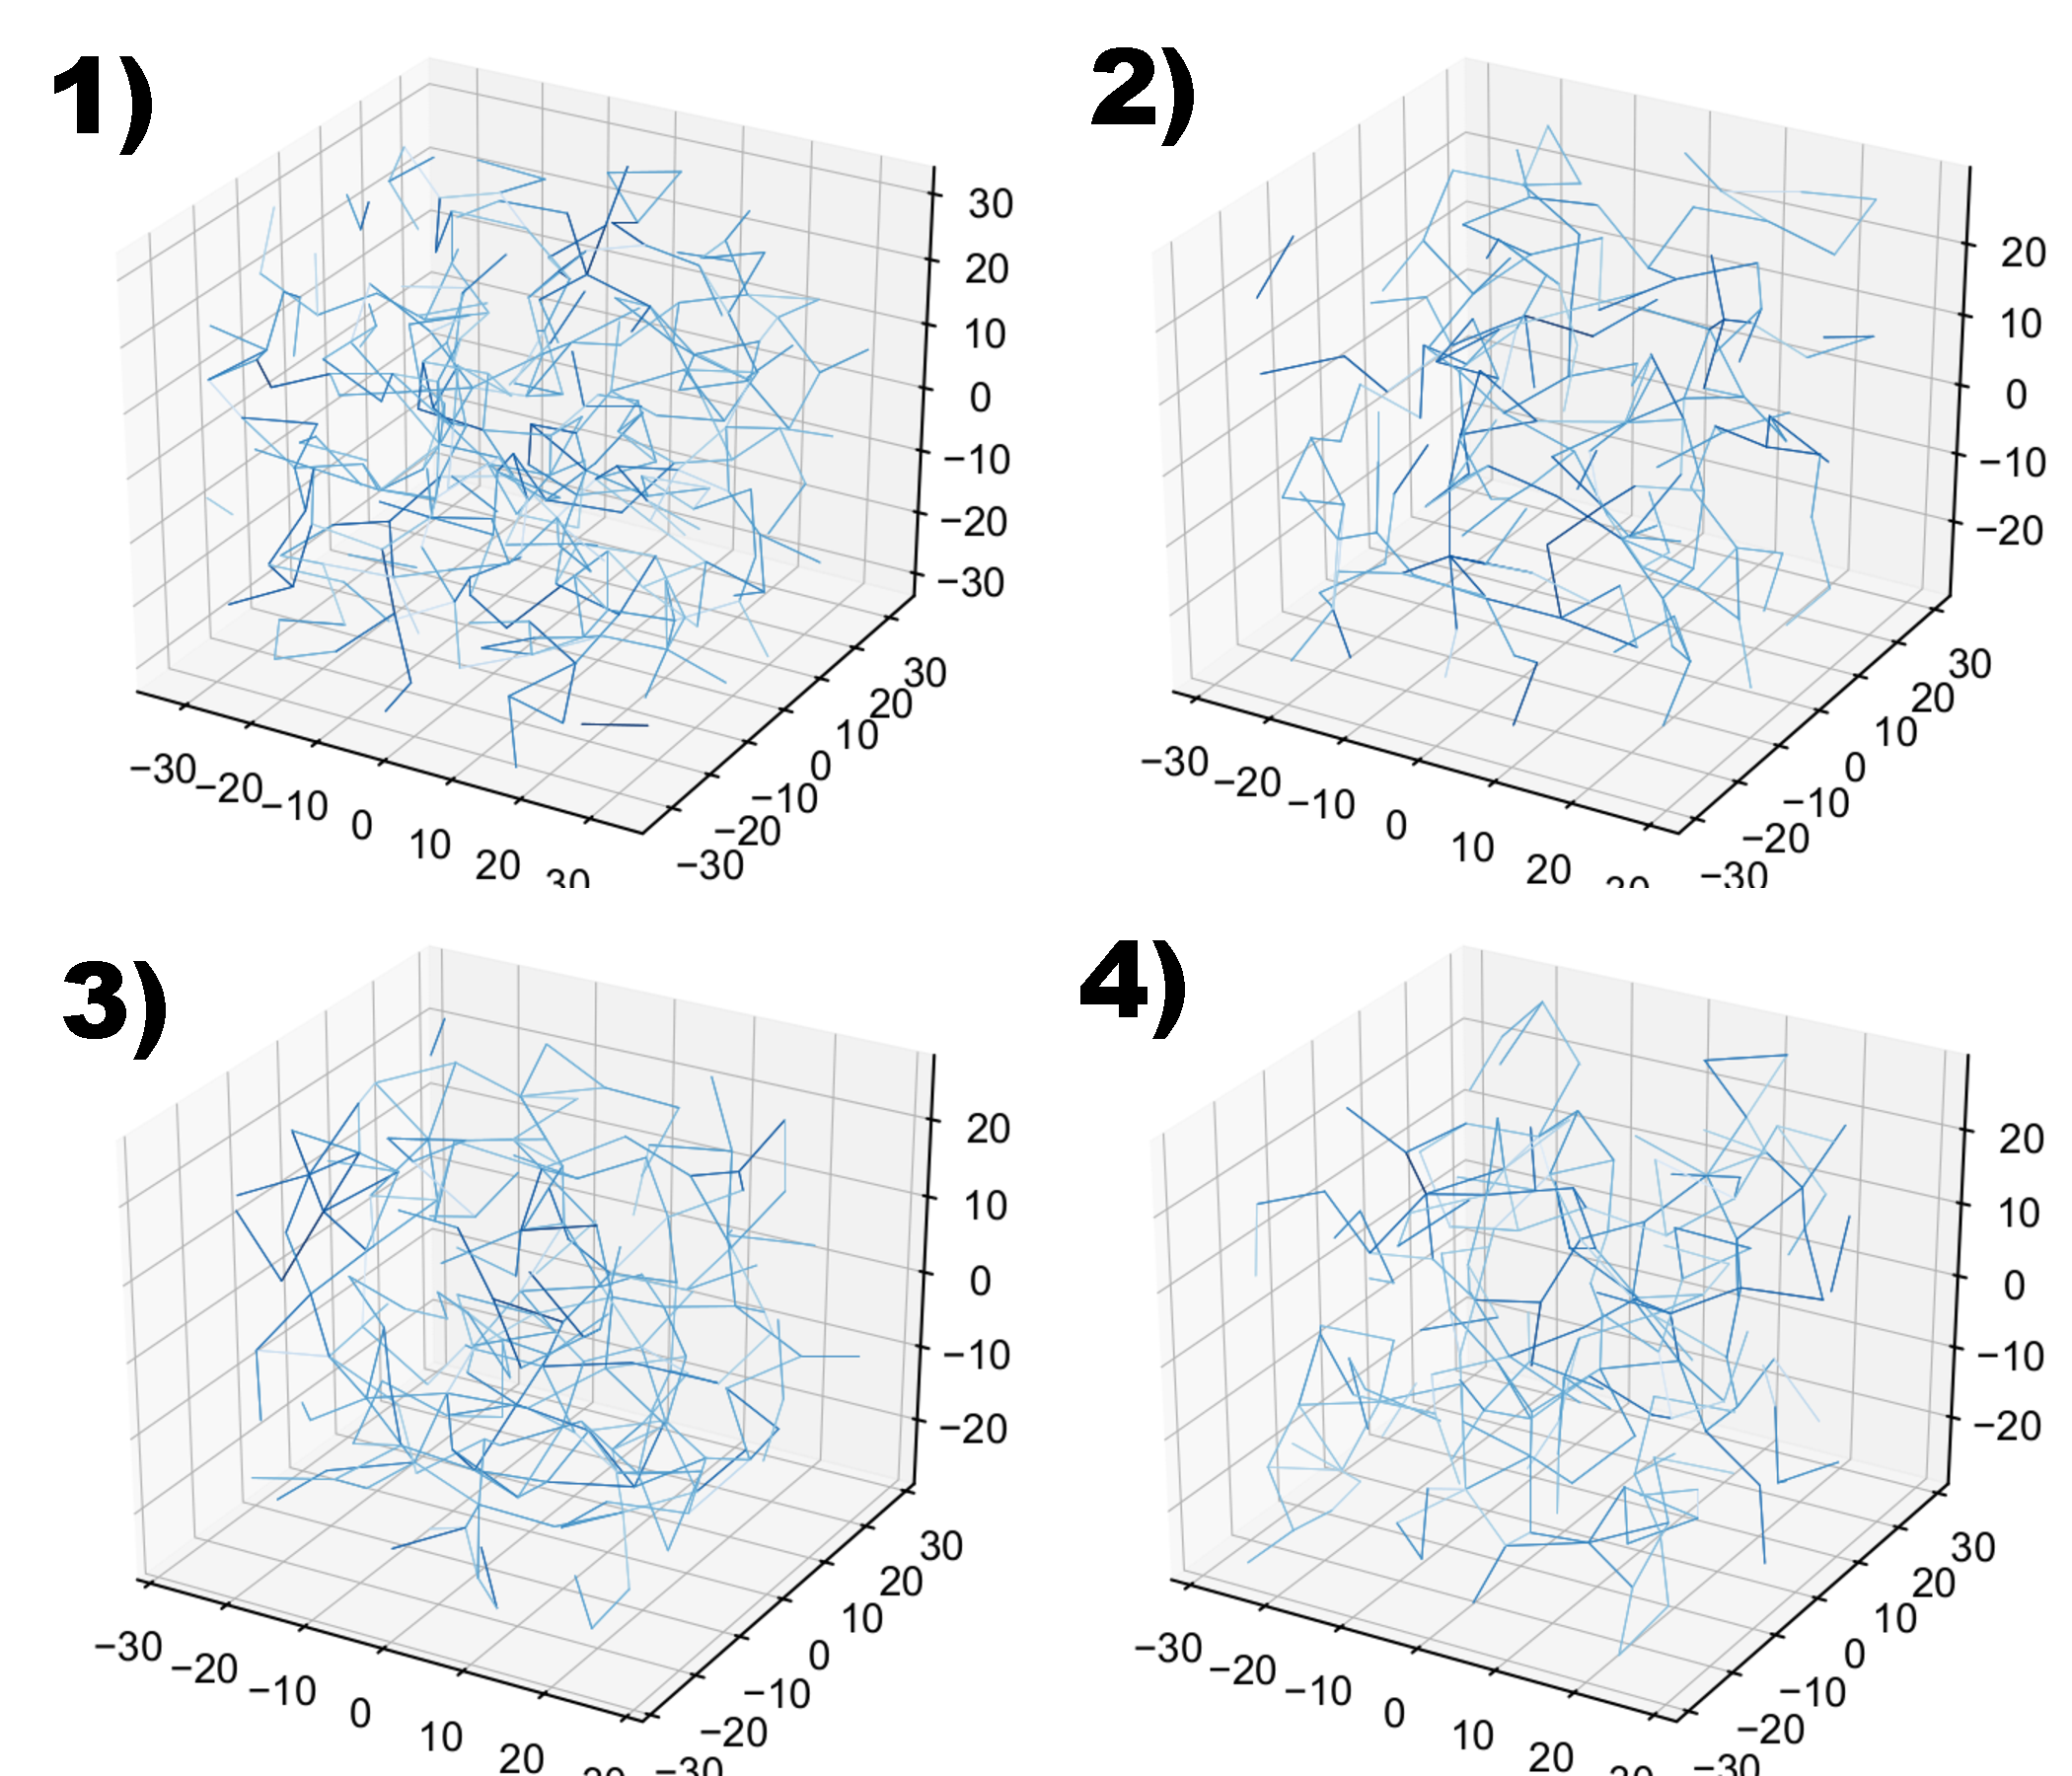
\includegraphics[width=\textwidth]{Figures/3dElectron.pdf}
    \caption{The 3D heatmap of charge transport routes within the morphologies \textbf{1} - \textbf{4}.
    Dark routes describe commonly accessed hops between pairs of chromophores, whereas pale routes are less widely used in the KMC simulations.
    Each node therefore represents the location of a single chromophore.
The intensity value for the route is currently taken to be \texttt{I $=$ np.log10(freq) $/$ np.log10(max\_freq)}.}
	\label{fig:3dNetwork}
\end{figure}

Nothing unusual to see here.

\begin{itemize}
    \item{\textbf{1} has more connections than the other 3 morphologies because there are more chromophores (300 compared to 200)}
    \item{Additionally, \textbf{1} has a larger proportion of dark blue routes in the middle of the morphology, which suggests that charge carriers are becoming trapped and just hopping between the same chromophores, accounting for the low recorded mobility.}
    \item{The most frequently-used routes in \textbf{4} are towards the edge and provide straight, linear paths from top-to-bottom and front-to-back of the morphology, which accounts for the high, anisotropic mobility.}
\end{itemize}


\clearpage


\subsection{MSDs}


\begin{figure}[h!]\centering
	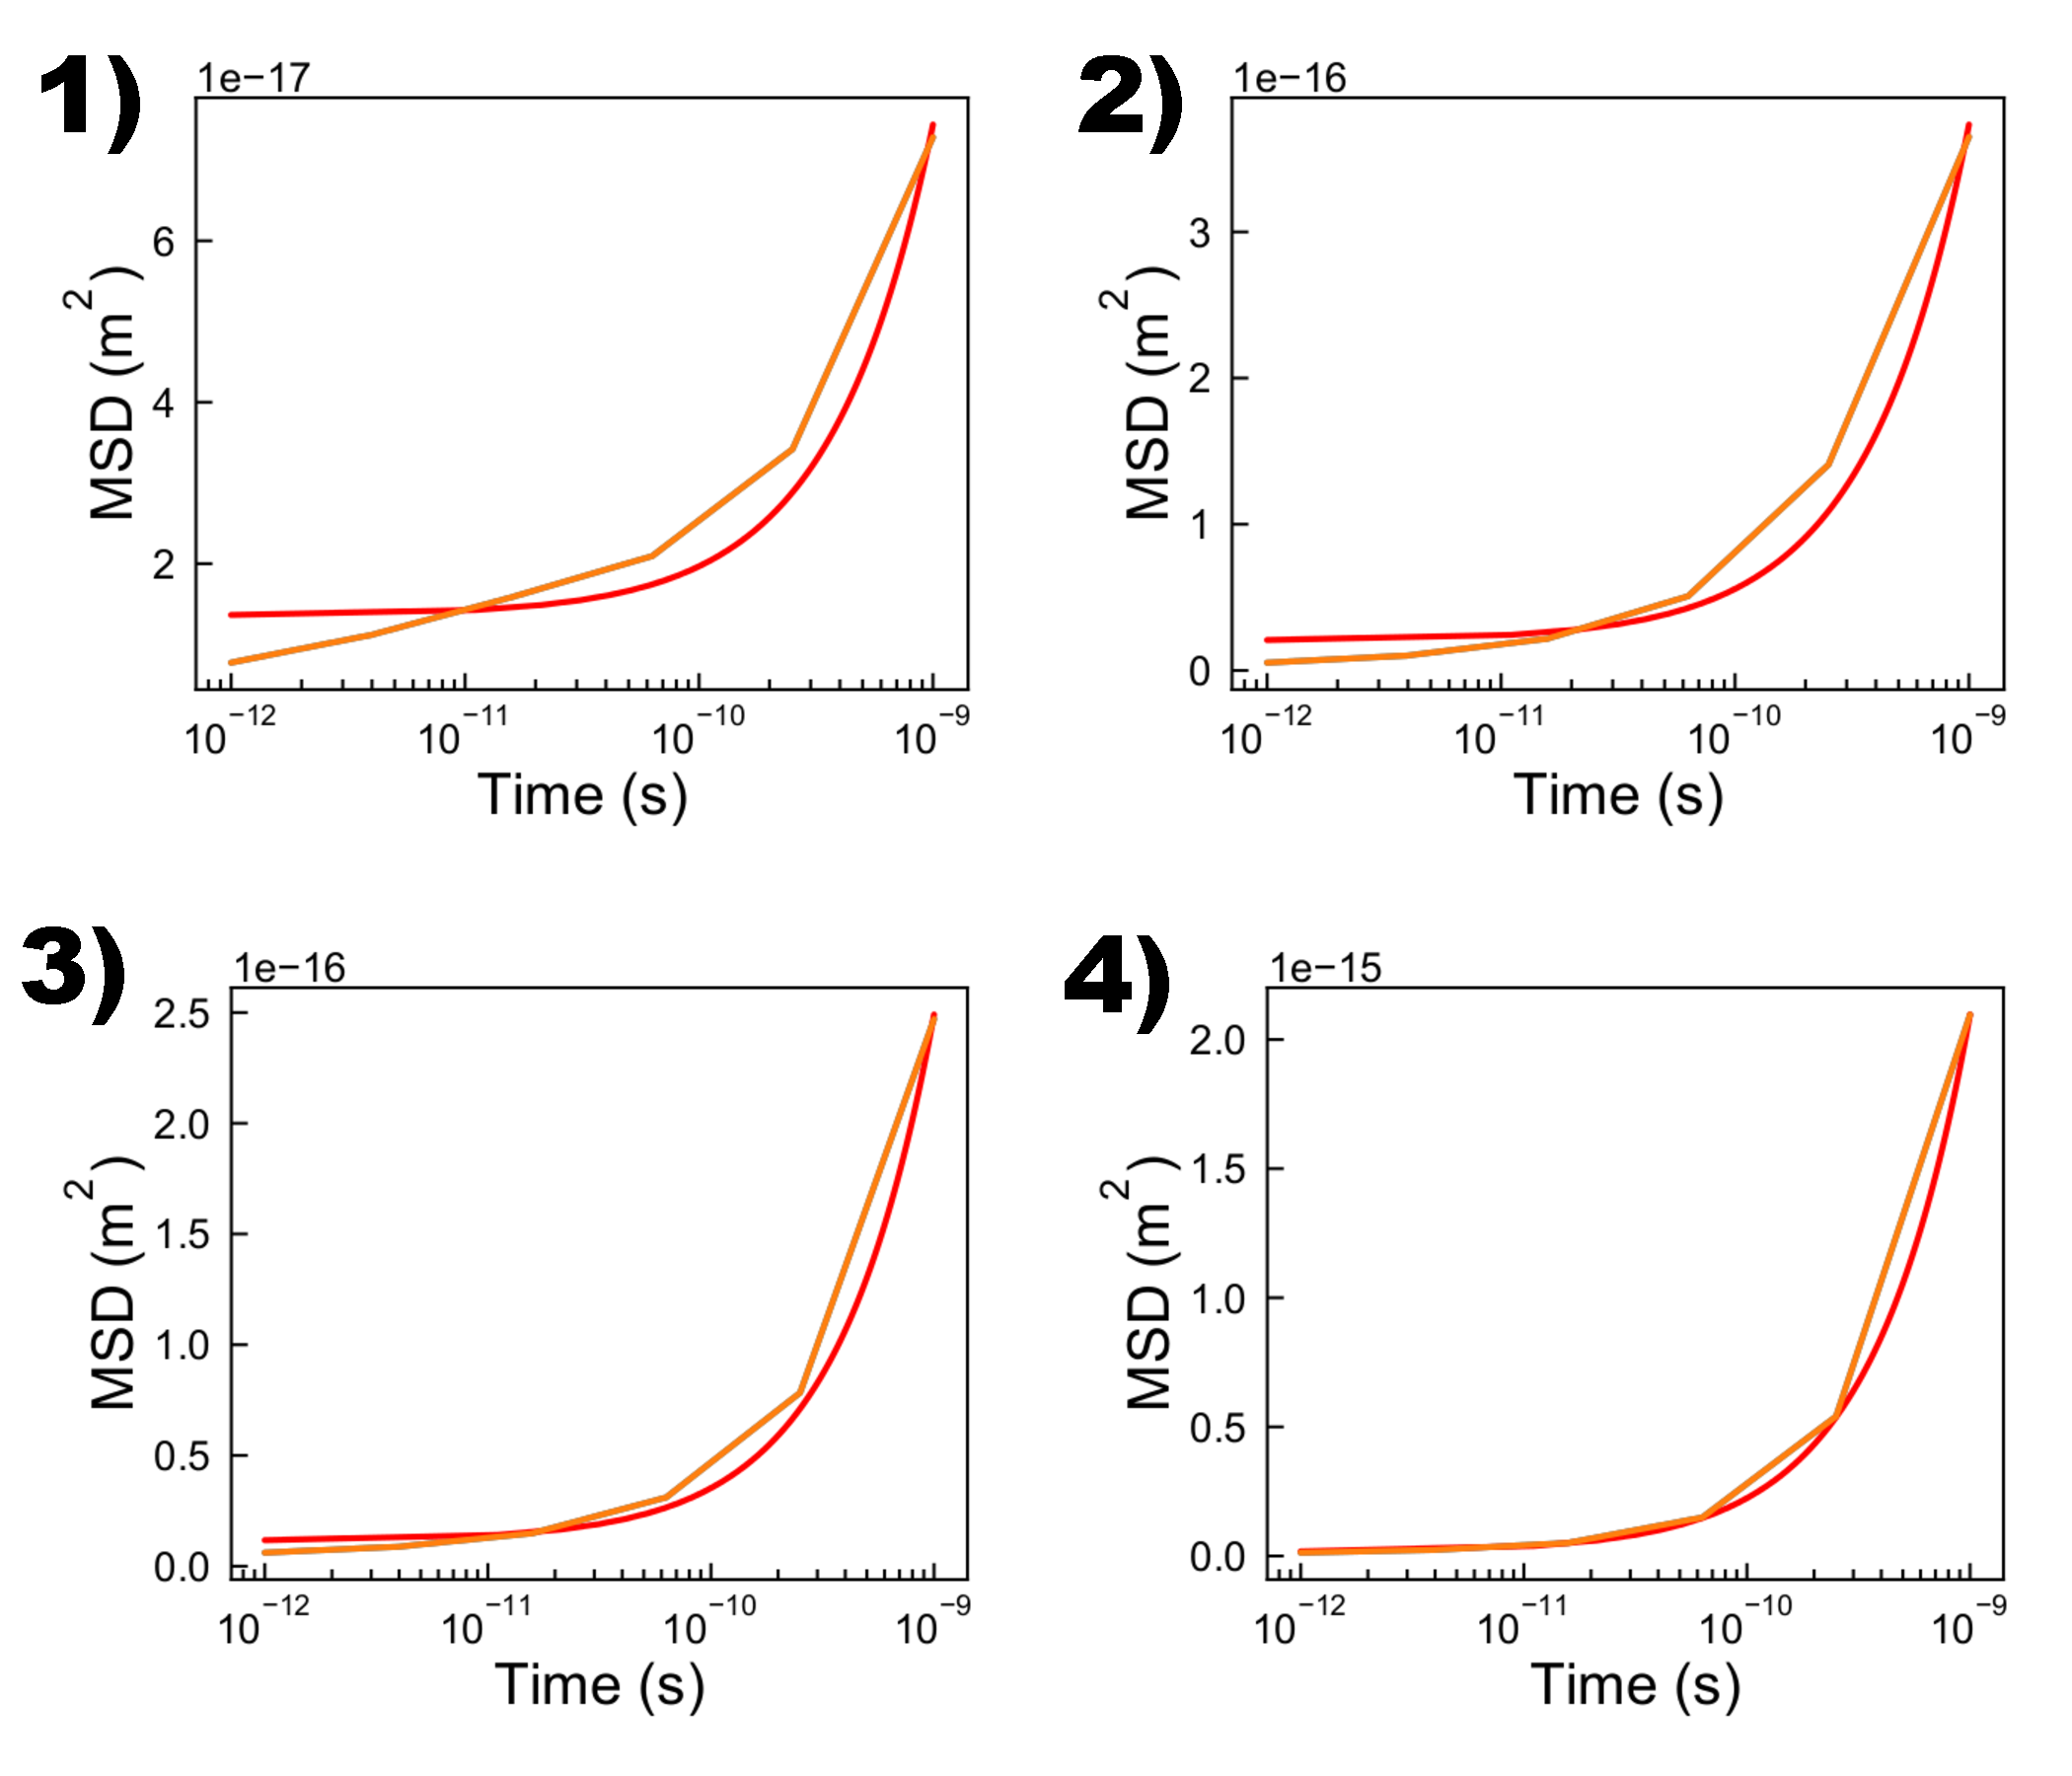
\includegraphics[width=\textwidth]{Figures/MSD.pdf}
    \caption{The semi-log-x mean squared displacement curves of the carriers within the morphologies \textbf{1} - \textbf{4}.
    The saturation behaviour observed on a linear axis with P3HT is also seen here, but to a lesser extent.
    All trendlines (red) have an $r^{2}$ correlation value of $>$ 99.9\%.}
	\label{fig:MSD}
\end{figure}


\begin{itemize}
    \item{The MSDs tend to exhibit the saturation behaviour (visible only on the linear scale) noted for the P3HT morphologies, but to a lesser extent.}
    \item{Fitting values vary from 98.51\% for \textbf{1}, through 99.21\% and 99.86\% for \textbf{2} and \textbf{3} respectively, up to 99.999\% for \textbf{4} (increased fitting accuracy at higher mobilities).} 
\end{itemize}


\clearpage


\section{Scattering Data}
 
\begin{figure}[h!]\centering
	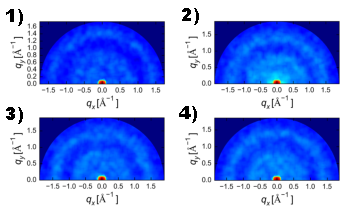
\includegraphics[width=\textwidth]{Figures/Scattering.pdf}
    \caption{Simulated scattering patterns of the morphologies \textbf{1} - \textbf{4}.
    Diffract has only been performed on the C0A atoms in the system that correspond to the fullerene C60 cage.}
	\label{fig:scattering}
\end{figure}


\begin{itemize}
    \item{The scattering patterns show two main features, a short-ranged structure peak at $\sim$ \SI{1.4}{\per\angstrom}, and a long-ranged peak at $<$ \SI{1}{\per\angstrom}.}
    \item{While I initially thought \textbf{4} was the `odd-one-out', it seems like actually \textbf{2}, \textbf{3} and \textbf{4} all have very similar diffraction patterns.}
    \item{Conversely, \textbf{1}'s short-ranged peak is significantly thinner than the other 3 morphologies, suggesting that the variation in short-range packing is less.
        \begin{itemize}
        \item{In general, I would expect this to lead to better charge transport, however, \textbf{1}'s mobility is significantly lower than the other 3 morphologies.}
        \item{It is difficult to compare the values directly though, as \textbf{1} contains 300 PCBM molecules, whereas the other 3 morphologies all contain 200 molecules.}
        \end{itemize}}
\end{itemize}

\clearpage

\section{Outstanding Questions}


\begin{itemize}
    \item{Where does the high mobility and beneficial connectivity in \textbf{4} come from, if there is no obvious difference in scattering patterns/packing between the 4 morphologies?}
    \item{How can two morphologies with the same density have 2 orders of magnitude difference in mobilities (\textbf{1} and \textbf{4}), but two morphologies with a near 20\% difference in density have a difference in mobility less than a factor of 2 (\textbf{2} and \textbf{3})?}
    \item{Is it just fluke that the connections in \textbf{4} run from one side of the morphology to the other, leading to fast mobilities and high anisotropies? What caused this?}
    \item{Why is there no clear temperature dependence, and why does the higher temperature morphology have higher mobility than the lower one in both cases?}
\end{itemize}


\bibliography{refs}
\bibliographystyle{unsrt}


\end{document}
